\documentclass[11pt, a4paper]{article}

\usepackage[top = 0.6 in, bottom = 0.6 in, left = 0.8 in, right = 0.8 in]{geometry}
\usepackage{amsmath, amssymb, amsfonts}

\allowdisplaybreaks[4]

\usepackage{enumerate}
\usepackage{array}
\usepackage{multirow}
\usepackage{dingbat}
\usepackage{fontawesome5}
\usepackage{tasks}
\usepackage{bbding}
\usepackage{undertilde}
\usepackage{twemojis}
% how to use bull's eye ----- \scalebox{2.0}{\twemoji{bullseye}}
\usepackage{fontspec}
\usepackage[colorlinks=true, linkcolor=blue]{hyperref}
\usepackage{fancyhdr}
\usepackage{lastpage}

\pagestyle{fancy}
\fancyhf{}
\fancyfoot[C]{Page \thepage\ of \pageref{LastPage}}
\renewcommand{\headrulewidth}{0pt}

\title{MSMS 402 : Assignment 02}
\author{{\fontsize{25}{20} \benyorithafont Ananda Biswas} \\[1em] Exam Roll No. : 24419STC053}
\date{\today}

\newfontface\benyorithafont{Benyoritha-G334D.otf}

\newfontface\myfont{Myfont1-Regular.ttf}[LetterSpace=0.05em]

\newfontface\cbfont{CaveatBrush-Regular.ttf}
% how to use --- \myfont --write text here--

\newfontface\gloriahallelujahfont{GLORIAHALLELUJAH-REGULAR.TTF}

\begin{document}

\maketitle

\section*{\textcolor{blue}{The Polar Method for Generating Normal Random Variables}}

Let $X$ and $Y$ be independent standard normal random variables and let $R$ and $\Theta$ denote the polar coordinates of the vector $(X, Y)$. That is (see Fig.~\ref{Figure1}),
\[
R^2 = X^2 + Y^2
\]
\[
\tan \Theta = \dfrac{Y}{X}
\]

\begin{figure}[!htbp]
\centering
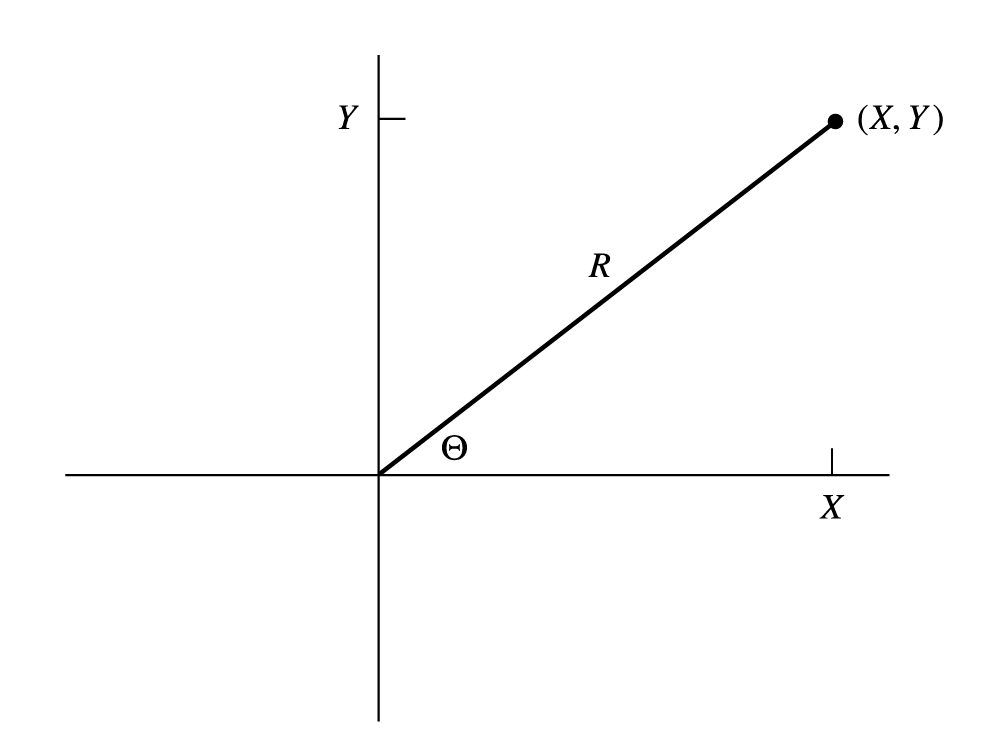
\includegraphics[scale=0.5]{figure1.png}
\caption{Polar coordinates}
\label{Figure1}
\end{figure}

Since $X$ and $Y$ are independent, their joint density is the product of their individual densities and is thus given by

\begin{align}\label{joint_pdf_xy}
f(x,y) 
&= \dfrac{1}{\sqrt{2\pi}} e^{-x^2/2} \cdot \dfrac{1}{\sqrt{2\pi}} e^{-y^2/2} \nonumber \\
&= \dfrac{1}{2\pi} e^{-(x^2 + y^2)/2}
\end{align}

To determine the joint density of $R^2$ and $\Theta$—call it $f(d,\theta)$—we make the change of variables
\[
d = x^2 + y^2, 
\qquad 
\theta = \tan^{-1}\!\left(\dfrac{y}{x}\right)
\]

As the Jacobian of this transformation—that is, the determinant of partial derivatives of $d$ and $\theta$ with respect to $x$ and $y$—is easily shown to equal $2$, it follows from Eq.\ (\ref{joint_pdf_xy}) that the joint density function of $R^2$ and $\Theta$ is given by
\[
f(d,\theta) = \dfrac{1}{2} \cdot \dfrac{1}{2\pi} e^{-d/2}, 
\qquad 0 < d < \infty,\; 0 < \theta < 2\pi
\]

However, as this is equal to the product of an exponential density having mean $2$ (namely, $\frac{1}{2} e^{-d/2}$) and the uniform density on $(0, 2\pi)$ [namely, $(2\pi)^{-1}$], it follows that

\begin{center}
$R^2$ and $\Theta$ are independent, with $R^2$ being exponential with mean $2$ and $\Theta$ being uniformly distributed over $(0, 2\pi)$.
\end{center}

We can now generate a pair of independent standard normal random variables $X$ and $Y$ by using the above to first generate their polar coordinates and then transform back to rectangular coordinates. This is accomplished as follows:

\begin{enumerate}[STEP 1:]
\item Generate random numbers $U_1$ and $U_2$.

\item $R^2 = -2 \log U_1$ (and thus $R^2$ is exponential with mean 2). $\Theta = 2\pi U_2$ and thus $\Theta$ is uniform between $0$ and $2\pi$).

\item Now let

\begin{align}\label{Box-Muller}
X &= R \cos \Theta = \sqrt{-2 \log U_1}\, \cos(2\pi U_2) \nonumber \\[0.2em]
Y &= R \sin \Theta = \sqrt{-2 \log U_1}\, \sin(2\pi U_2).
\end{align}
\end{enumerate}

The transformations given by Eqs. (\ref{Box-Muller}) are known as the \textbf{Box-Muller transformations}. \\[0.5em]

Unfortunately, the use of the Box--Muller transformations (\ref{Box-Muller}) to generate a pair of independent standard normals is computationally not very efficient. The reason for this is the need to compute the sine and cosine trigonometric functions. There is, however, a way to get around this time-consuming difficulty by an indirect computation of the sine and cosine of a random angle (as opposed to a direct computation which generates $U$ and then computes the sine and cosine of $2\pi U$). To begin, note that if $U$ is uniform on $(0,1)$, then $2U$ is uniform on $(0,2)$, and so $2U - 1$ is uniform on $(-1,1)$. Thus, if we generate random numbers $U_1$ and $U_2$ and set
\[
V_1 = 2U_1 - 1
\]
\[
V_2 = 2U_2 - 1
\]
then $(V_1, V_2)$ is uniformly distributed in the square of area $4$ centered at $(0,0)$---see Fig.~\ref{Figure2}.

\begin{figure}
\centering
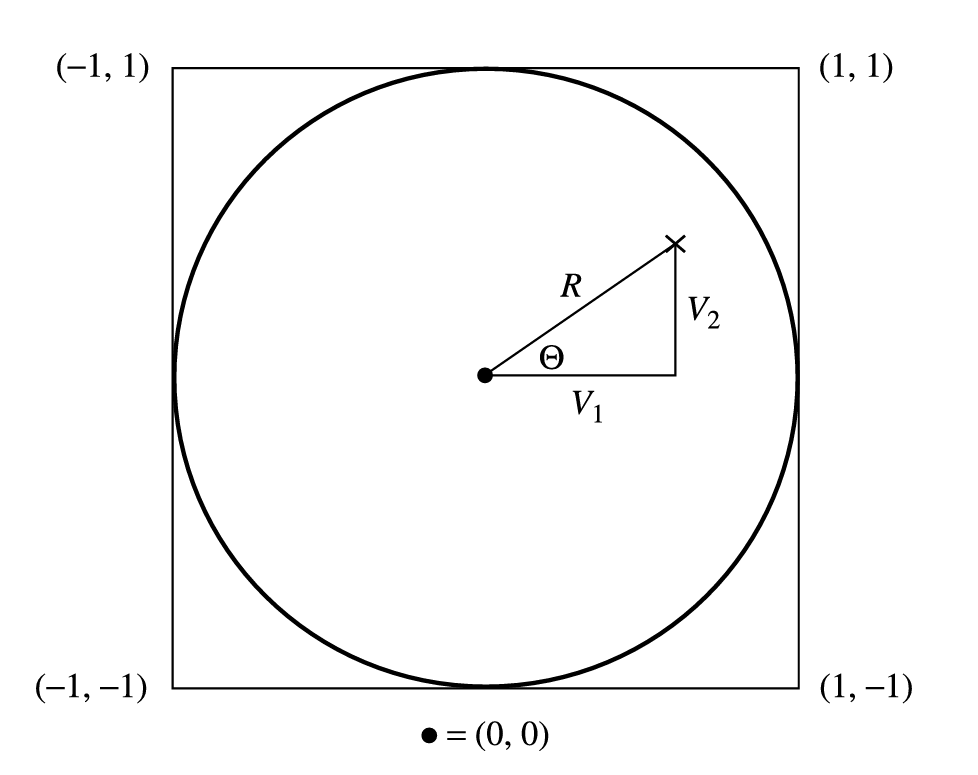
\includegraphics[scale=0.5]{figure2.png}
\caption{$(V_1, V_2)$ uniformly distributed in the square}
\label{Figure2}
\end{figure}

\vspace{0.5em}

Suppose now that we continually generate such pairs $(V_1, V_2)$ until we obtain one that is contained in the circle of radius $1$ centered at $(0,0)$---that is, until $(V_1, V_2)$ is such that
\[
V_1^2 + V_2^2 \leq 1.
\]

It now follows that such a pair $(V_1, V_2)$ is uniformly distributed in the circle. If we let $R$ and $\Theta$ denote the polar coordinates of this pair, then it is not difficult to verify that $R$ and $\Theta$ are independent, with $R^2$ being uniformly distributed on $(0,1)$ and with $\Theta$ being uniformly distributed over $(0, 2\pi)$. Since $\Theta$ is thus a random angle, it follows that we can generate the sine and cosine of a random angle $\Theta$ by generating a random point $(V_1, V_2)$ in the circle and then setting
\[
\sin \Theta = \dfrac{V_2}{R} = \dfrac{V_2}{\left(V_1^2 + V_2^2\right)^{1/2}}
\]
\[
\cos \Theta = \dfrac{V_1}{R} = \dfrac{V_1}{\left(V_1^2 + V_2^2\right)^{1/2}}
\]

It now follows from the Box--Muller transformation (\ref{Box-Muller}) that we can generate independent standard normals by generating a random number $U$ and setting
\begin{align}\label{X_Y_new}
X &= \left(-2 \log U \right)^{1/2} \dfrac{V_1}{\left(V_1^2 + V_2^2\right)^{1/2}} \nonumber \\[0.5em]
Y &= \left(-2 \log U \right)^{1/2} \dfrac{V_2}{\left(V_1^2 + V_2^2\right)^{1/2}}.
\end{align}

In fact, since $R^2 = V_1^2 + V_2^2$ is itself uniformly distributed over $(0,1)$ and is independent of the random angle $\Theta$, we can use it as the random number $U$ needed in Eqs.\ (\ref{X_Y_new}). Therefore, letting $S = R^2$, we obtain that
\[
X = \left(-2 \log S \right)^{1/2} \dfrac{V_1}{S^{1/2}} 
= V_1 \left( \dfrac{-2 \log S}{S} \right)^{1/2}
\]
\[
Y = \left(-2 \log S \right)^{1/2} \dfrac{V_2}{S^{1/2}} 
= V_2 \left( \dfrac{-2 \log S}{S} \right)^{1/2}
\]

are independent standard normals when $(V_1, V_2)$ is a randomly chosen point in the circle of radius $1$ centered at the origin, and $S = V_1^2 + V_2^2$.

Summing up, we thus have the following approach to generating a pair of independent standard normals:

\begin{enumerate}[STEP 1:]
\item Generate random numbers $U_1$ and $U_2$.
    
\item Set $V_1 = 2U_1 - 1$, \quad $V_2 = 2U_2 - 1$, \quad $S = V_1^2 + V_2^2$.
    
\item If $S > 1$, return to Step 1.
    
\item Return the independent standard normals:
    \[
    X = \sqrt{\dfrac{-2 \log S}{S}}\, V_1, 
    \qquad
    Y = \sqrt{\dfrac{-2 \log S}{S}}\, V_2
    \]
\end{enumerate}

The above is called the \textbf{polar method}. Since the probability that a random point in the square will fall within the circle is equal to $\pi/4$ (the area of the circle divided by the area of the square), it follows that, on average, the polar method will require $4/\pi = 1.273$ iterations of Step $1$. Hence it will, on average, require $2.546$ random numbers, $1$ logarithm, $1$ square root, $1$ division, and $4.546$ multiplications to generate two independent standard normals.


\end{document}